\documentclass[a4paper]{article}
\usepackage[utf8]{inputenc}
\usepackage[T1]{fontenc}
\usepackage[french]{babel}
\usepackage{geometry}
\geometry{hmargin=3.5cm,vmargin=3.5cm}
\usepackage{graphicx}
\usepackage[nottoc, notlof, notlot]{tocbibind}

%% \usepackage[vlined, lined, linesnumbered, boxruled, french]{algorithm2e}
\usepackage{fancyhdr}
\pagestyle{fancy}

\lhead{Background}
\rhead{Simulateur de caches multi-c\oe ur}
\lfoot{ENSEIRB-MATMECA}
\rfoot{PFA 2013-2014}

\begin{document}

\thispagestyle{empty}

\vspace{\stretch{1}}
\hrule
\begin{flushleft}
\huge{Simulateur de caches sur\\architecture multi-c\oe ur :}\\
\end{flushleft}
\begin{flushright}
\Huge\textbf{Rapport}\\
\end{flushright}
\hrule

\vspace{\stretch{1}}
\noindent\textbf{Auteurs :}
\emph{DUBOIS Nicolas, GOUDET Pierre, HENG Nicolas, HONORAT Alexandre, MARAIT Gilles, PICHON Grégoire}\\
\\
\noindent\textbf{Client :}
\emph{M. BARTHOU Denis}\\
\\
\noindent\textbf{Responsable pédagogique :}
\emph{M. MORANDAT Floréal} 

\vspace{\stretch{1}}
\normalsize
\begin{center}
  Deuxième année, filière informatique\\
  Date : \today\\
  \textsc{Enseirb-Matmeca}
\end{center}


\newpage
\tableofcontents

\newpage
\section*{Introduction}

\indent Dernièrement la vitesse des processeurs a considérablement augmenté (loi de Moore) alors que le temps d'accès à la mémoire RAM (Random-Access Memory) est resté globalement le même. Pour permettre d'accèder rapidement à des éléments mémoire non contenus dans les registres, des caches sont utilisés. Cette organisation hiérarchique a plusieurs objectifs: \\
\begin{itemize}
\item Etre assez conséquente en termes de taille pour pouvoir contenu la totalité de l'espace adressable.
\item Etre organisée de manière à être rapide.
\item Ne pas coûter trop cher. \\
\end{itemize}

\indent Les caches permettent de stocker la mémoire utilisée récemment dans les registres, en se basant sur deux concepts: la localité spatiale et la localité temporelle. La localité temporelle est l'idée qu'une cellule mémoire accédée récemment soit de nouveau utilisée dans un futur proche. La localité spatiale est l'idée que si l'on accède à une cellule mémoire $X$, la cellule mémoire $X+1$ a de grandes chances d'être utilisée. \\

\indent Les mémoires de haut niveau, proches du processeur, sont généralement de petite taille. Leur coût est conséquent mais leur accès est très rapide. On peut résumer comme suit une hiérarchie mémoire classique: \\

\begin{figure}[!h]
\begin{center}
   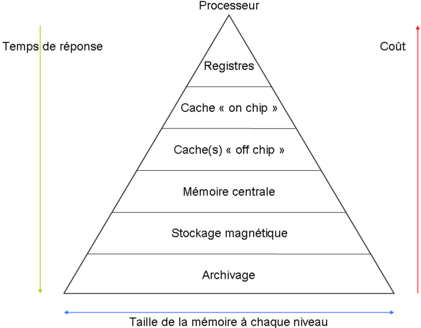
\includegraphics[scale=0.75]{hierarchy.png}
   \caption{\label{hierarchy} Hiérachie mémoire}
\end{center}
\end{figure}

\newpage
\nocite{*}
\bibliographystyle{plain}
\bibliography{rapport}

\end{document}
